\documentclass[12pt]{article}

% --- Preamble ---
\usepackage[utf8]{inputenc}
\usepackage[T1]{fontenc}
\usepackage{lmodern}
\usepackage{amsmath, amssymb}
\usepackage{graphicx}
\usepackage{geometry}
\geometry{a4paper, margin=1in}
\usepackage{hyperref} % For clickable links
\usepackage{caption} % For figure and table captions
\usepackage{subcaption} % For subfigures
\usepackage{float}

% --- Document Information ---
\title{Research Report Title}
\author{Your Name(s) \\ Your Affiliation(s) \\ Your Email Address(es)}
\date{\today}

% --- Abstract Environment ---
\usepackage{abstract}
\renewcommand{\abstractname}{Abstract}

% --- Sections and Subsections ---
\setcounter{secnumdepth}{2} % Number up to subsections
\setcounter{tocdepth}{2}    % Include up to subsections in the table of contents

% --- Begin Document ---
\begin{document}

% --- Title Page ---
\maketitle
\begin{abstract}
This section provides a concise summary of your research report. It should briefly outline the problem, the methods used, the key findings, and the main conclusions. Keep it brief and impactful.
\end{abstract}

% --- Table of Contents ---
\tableofcontents
\newpage

% --- Introduction ---
\section{Introduction}
\label{sec:introduction}
This section should introduce the research topic, provide necessary background information, state the problem or research question, and outline the objectives and scope of the report.

% --- Methods ---
\section{Methods}
\label{sec:methods}

\subsection{Participants}
\label{subsec:participants}
This study analyzed responses from a total of 43 college students, the majority of whom were enrolled at the University of Florida. While demographic details such as age and gender were not collected, participants were asked to self-identify their academic major by selecting one of six broad categories: Engineering, Business, Liberal Arts and Sciences, Health Professions, Law Professions, and Agriculture. These categories were chosen to capture a diverse range of academic disciplines. However, this categorization may have obscured differences between individual majors within a given category, presenting a limitation in the analysis of discipline-specific trends.

\subsection{Instruments}
\label{subsec:instruments}
To examine how AI usage patterns differ across academic disciplines, a five-question survey was developed to collect both quantitative and qualitative data. The first question asked participants to indicate their academic discipline using the predefined categories. The second assessed the frequency of AI use for academic purposes, using a five-point Likert scale ranging from “never” to “daily.”
The third question asked students to select from a list of AI tools and services they had used for academic purposes, including options such as ChatGPT, Grammarly, Claude, and others. The fourth question addressed the specific academic tasks for which students used AI, such as writing assignments, coding, research, or exam preparation.
The final question consisted of three attitudinal statements rated on a five-point Likert scale, ranging from “strongly disagree” to “strongly agree”. These statements gauged students’ perceptions of AI’s educational value, accessibility, and its relevance to their particular field of study.
Together, these items were designed to capture both the behaviors and perceptions of students engaging with AI tools in their academic work. A copy of the full survey is included in the Appendix.


\subsection{Procedure}
\label{subsec:procedure}
The survey was administered through Qualtrics and distributed electronically over a one-week period. Recruitment was conducted via university-affiliated group chats and social media platforms to reach a wide range of students across disciplines.
Early in the distribution process, it became evident that responses were heavily skewed toward Engineering majors. To address this imbalance, targeted efforts were made to gather more responses from underrepresented fields. Despite these efforts, Engineering remained overrepresented, accounting for 46% of the sample. This disproportion is acknowledged as a limitation when interpreting the findings.
Following data collection, responses were cleaned and analyzed using both Qualtrics and Python’s Pandas library.




% --- Results ---
\section{Results}
Of the 43 total respondents, Engineering students made up the largest group with 18 participants, followed by 11 from Liberal Arts and Sciences, 5 each from Business and Health Professions, and 4 whose majors did not align with the listed categories (Figure 1).


\begin{figure}[htbp]
  \centering
  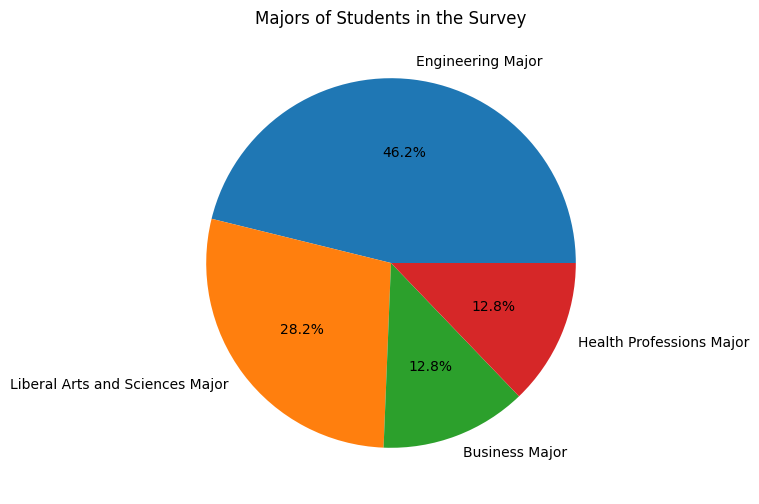
\includegraphics[width=0.6\textwidth]{fig1.png} % Replace with your figure file name
  \caption{A brief description of the figure.}
  \label{fig:example1}
\end{figure}

All participants reported using AI tools for academic purposes at least a few times per month. The most common frequency was “a few times per week,” selected by 15 participants. Nine reported using AI “nearly every day,” seven used it “daily,” and another seven indicated use “at least once a week.” No respondents selected “never” or “a few times a month,” indicating consistent and regular engagement with AI tools across the sample (Figure 2).

\begin{figure}[htbp]
  \centering
  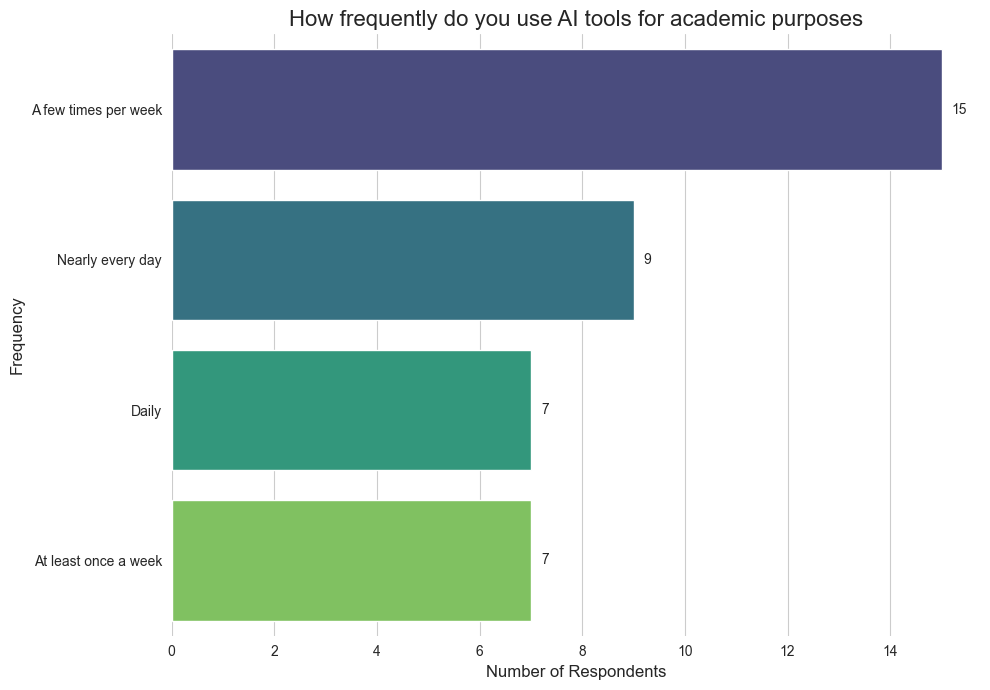
\includegraphics[width=0.6\textwidth]{fig2.png} % Replace with your figure file name
  \caption{A brief description of the figure.}
  \label{fig:example1}
\end{figure}

ChatGPT was by far the most widely used tool, reported by 38 out of 39 respondents (97\%). Gemini followed at 46\%, with other tools including Grammarly AI (26\%), Claude (23\%), DALL·E (15\%), and DeepSeek (13\%). Grok and GitHub Copilot were the least used, each mentioned by only one respondent (3\%) (Figure 3).

\begin{figure}[htbp]
  \centering
  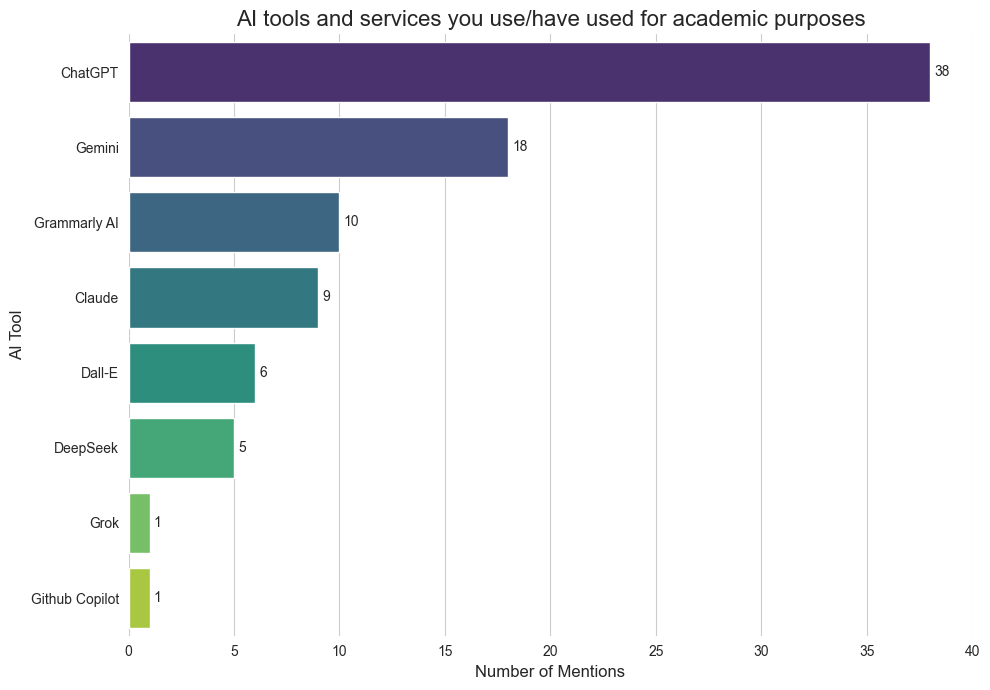
\includegraphics[width=0.65\textwidth]{fig3.png} % Replace with your figure file name
  \caption{A brief description of the figure.}
  \label{fig:example1}
\end{figure}

Breakdowns of AI tool usage by major (Figure 4) suggested differences in tool preference across disciplines. Among Engineering majors, 94\% reported using ChatGPT, with 39\% using Gemini and 28\% using Claude. In Liberal Arts and Sciences, all 11 participants reported using ChatGPT, 46\% used Gemini, and 27\% used Grammarly. While these patterns suggest some variation, limited sample sizes in several categories constrain broader generalizations.

% Example of two subfigures side-by-side
\begin{figure}[H]
  \centering
  \begin{subfigure}[b]{0.45\textwidth}
    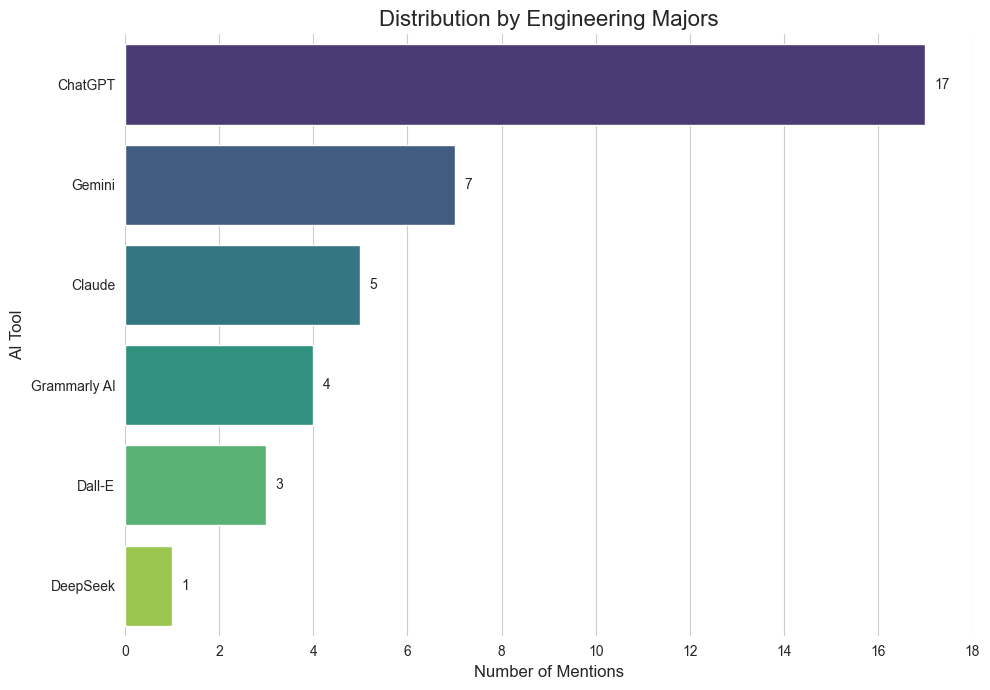
\includegraphics[width=\textwidth]{fig4-1.png} % Replace with your first subfigure file name
    %\caption{Description of subfigure (a)}
    \label{fig:subfig1a}
  \end{subfigure}
  \hfill % Add some horizontal space between the subfigures
  \begin{subfigure}[b]{0.45\textwidth}
    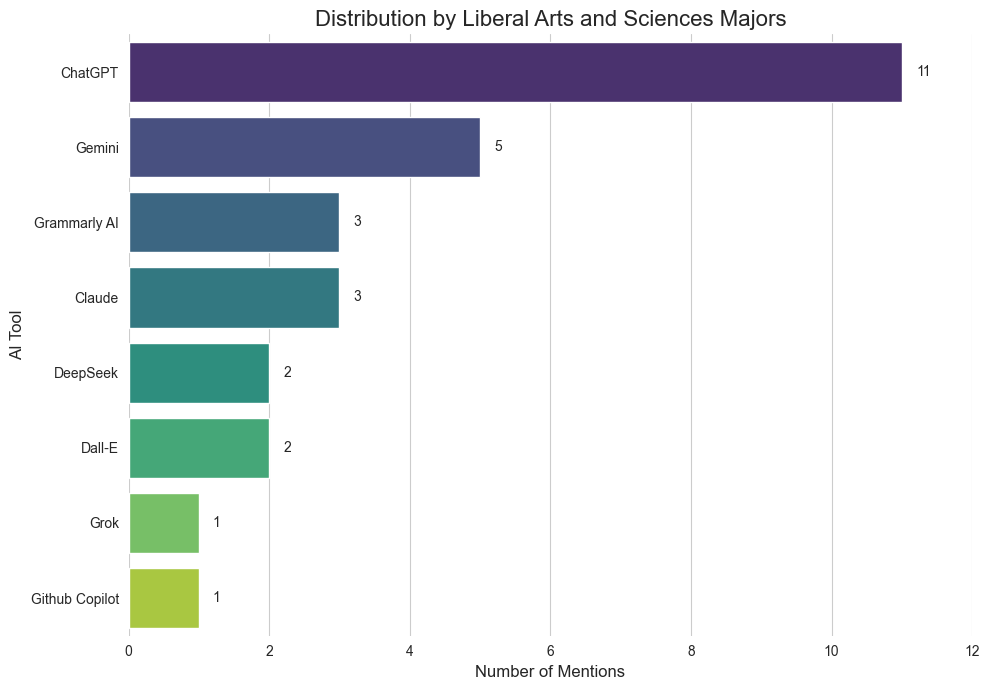
\includegraphics[width=\textwidth]{fig4-2.png} % Replace with your second subfigure file name
    %\caption{Description of subfigure (b)}
    \label{fig:subfig1b}
  \end{subfigure}
  \hfill % Add some horizontal space between the subfigures
  \begin{subfigure}[b]{0.45\textwidth}
    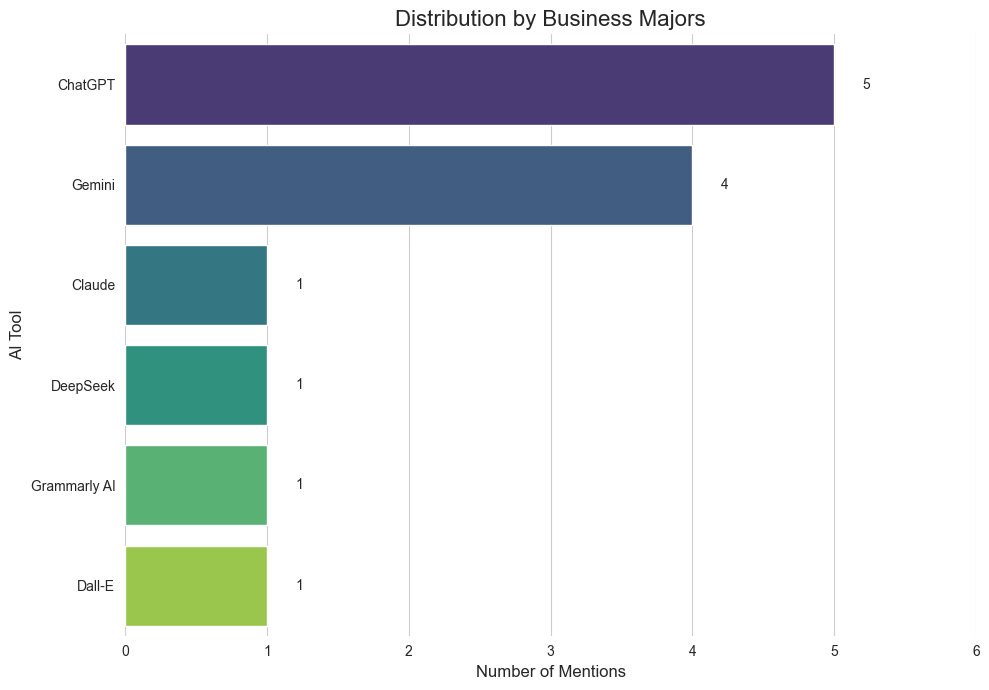
\includegraphics[width=\textwidth]{fig4-3.png} % Replace with your second subfigure file name
    %\caption{Description of subfigure (b)}
    \label{fig:subfig1b}
  \end{subfigure}
  \hfill % Add some horizontal space between the subfigures
  \begin{subfigure}[b]{0.45\textwidth}
    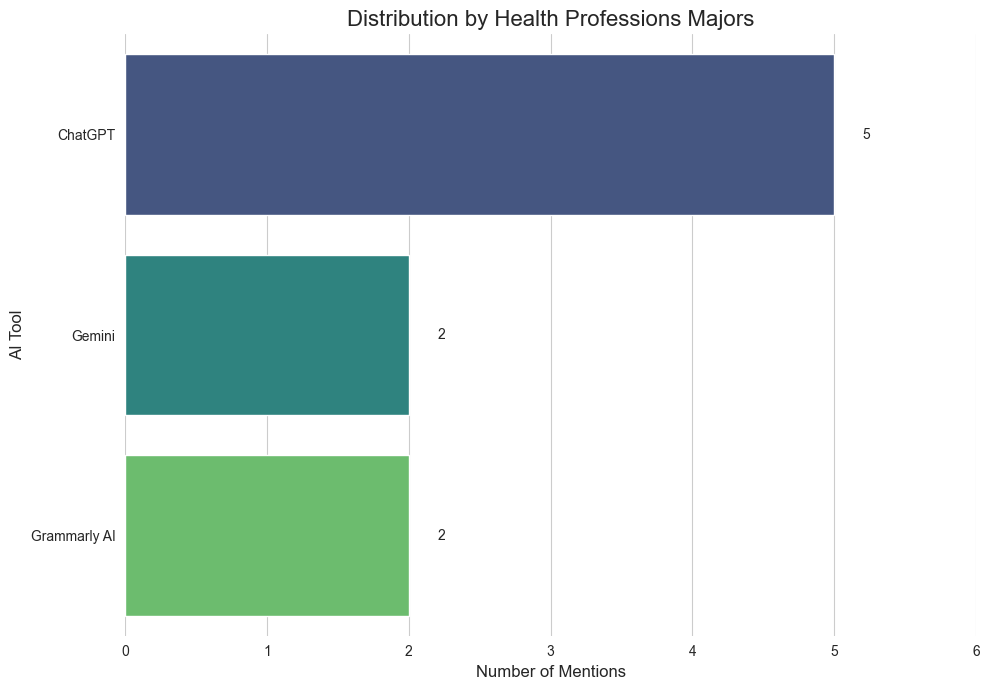
\includegraphics[width=\textwidth]{fig4-4.png} % Replace with your second subfigure file name
    %\caption{Description of subfigure (b)}
    \label{fig:subfig1b}
  \end{subfigure}
  \caption{Overall caption for the two subfigures.}
  \label{fig:subfigures1}
\end{figure}


Participants reported using AI for a wide variety of academic tasks. Writing and editing was the most frequently cited use, selected by 87\% of respondents. Other common applications included research and information gathering (74\%), studying and note-taking (62\%), and math or problem solving (59\%). Additional uses included career development (46\%), coding (41\%), productivity and organization (26\%), data analysis (21\%), and content creation (18\%) (Figure 5).


\begin{figure}[htbp]
  \centering
  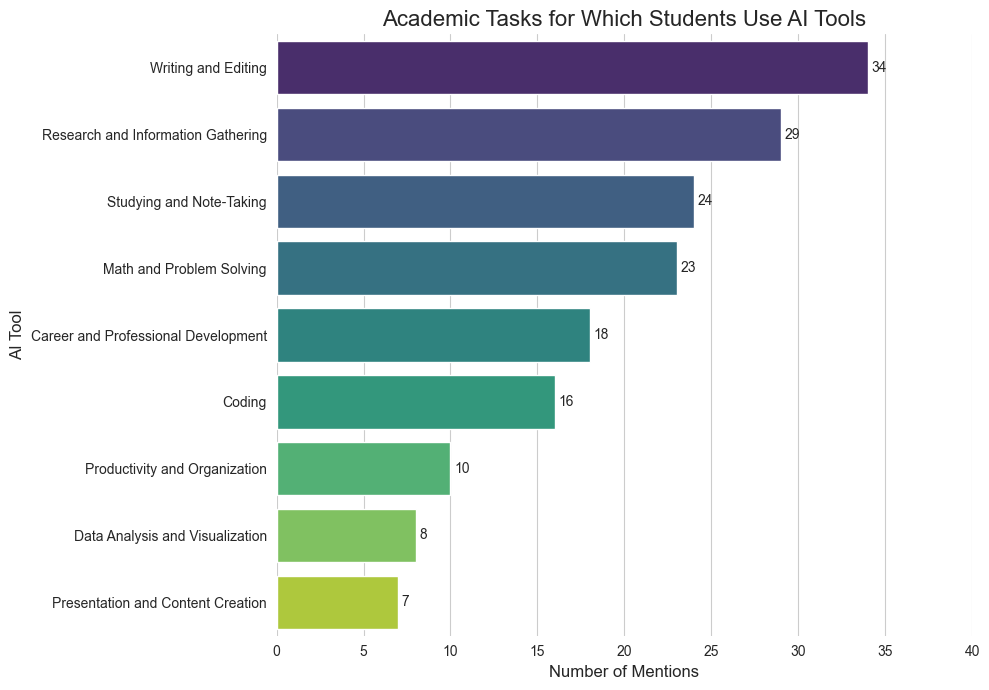
\includegraphics[width=0.5\textwidth]{fig5.png} % Replace with your figure file name
  \caption{A brief description of the figure.}
  \label{fig:example1}
\end{figure}

Figure 6 provides further detail on how usage patterns differed by academic discipline. For example, coding was a more frequent use case among Engineering majors, while writing and research were broadly cited across all fields.

% Example of two subfigures side-by-side
\begin{figure}[H]
  \centering
  \begin{subfigure}[b]{0.45\textwidth}
    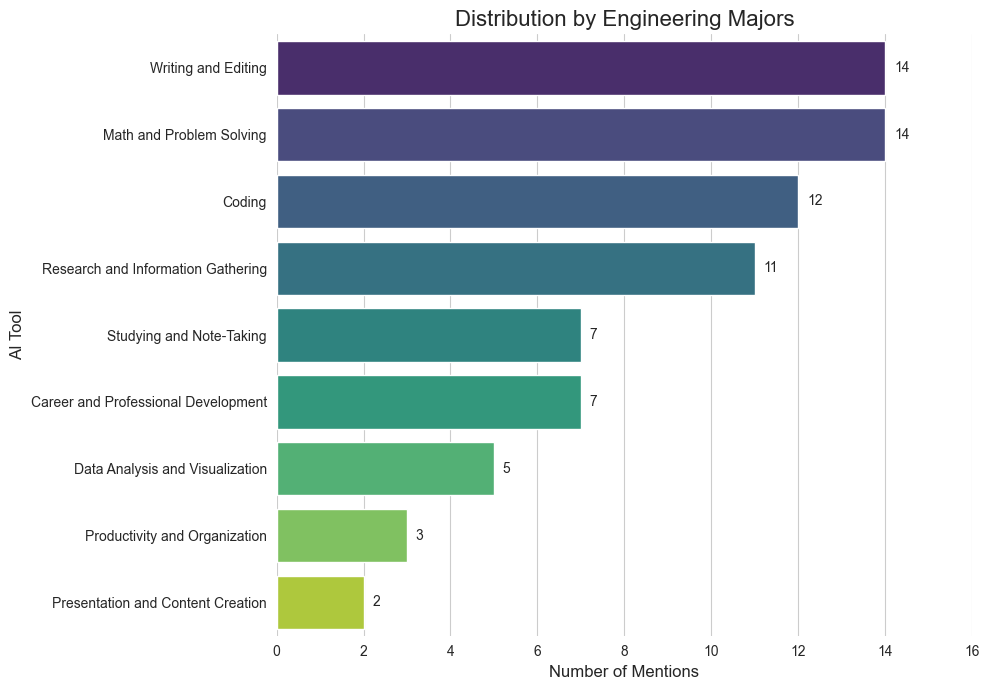
\includegraphics[width=\textwidth]{fig6-1.png} % Replace with your first subfigure file name
    %\caption{Description of subfigure (a)}
    \label{fig:subfig1a}
  \end{subfigure}
  \hfill % Add some horizontal space between the subfigures
  \begin{subfigure}[b]{0.45\textwidth}
    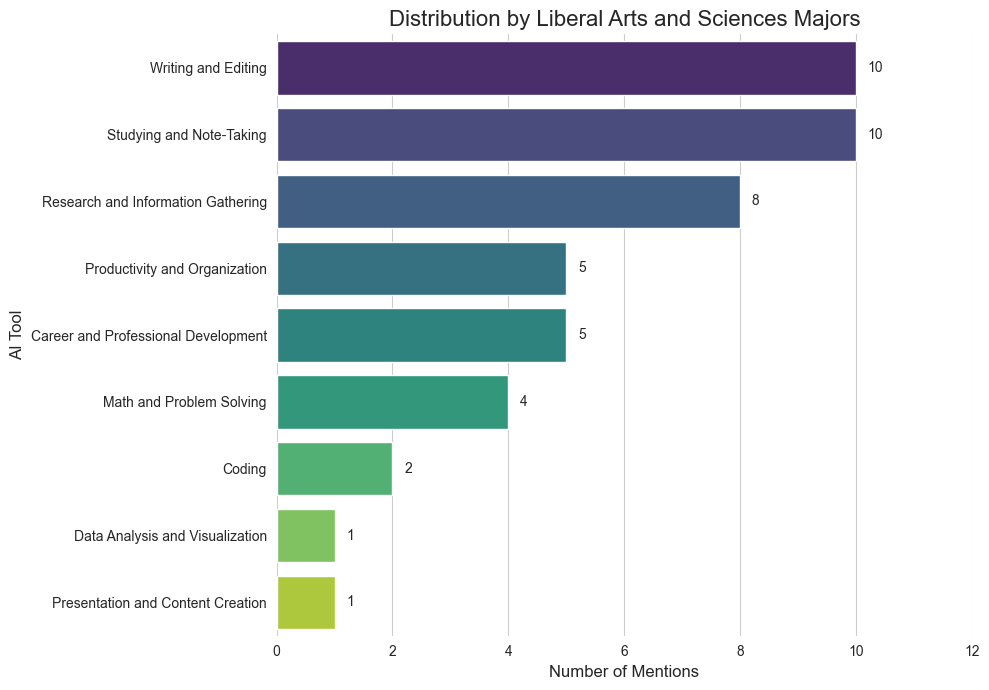
\includegraphics[width=\textwidth]{fig6-2.png} % Replace with your second subfigure file name
    %\caption{Description of subfigure (b)}
    \label{fig:subfig1b}
  \end{subfigure}
  \hfill % Add some horizontal space between the subfigures
  \begin{subfigure}[b]{0.45\textwidth}
    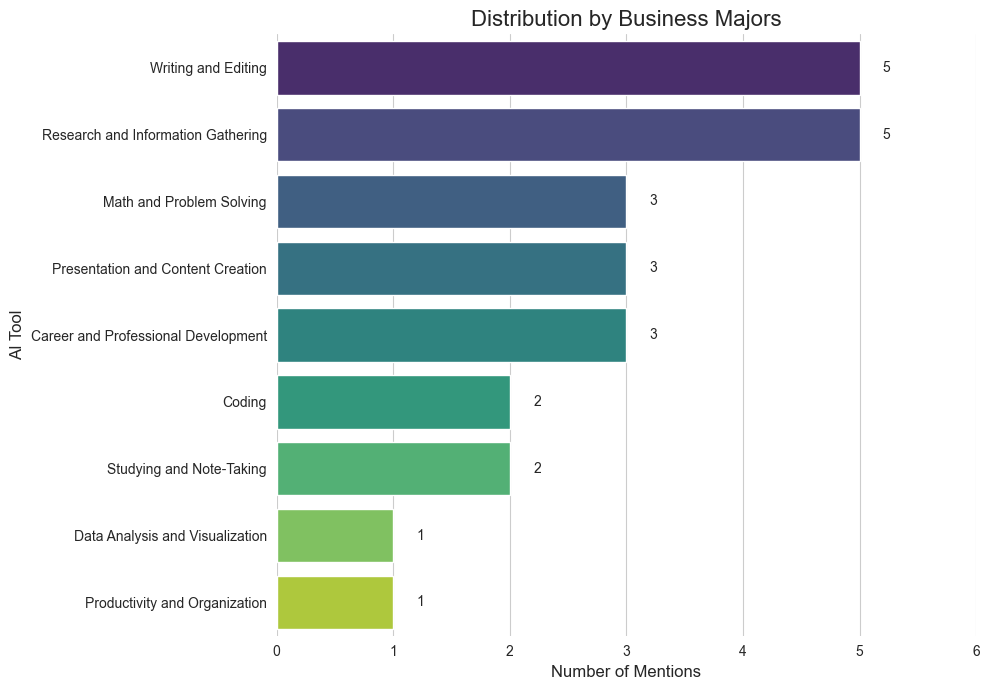
\includegraphics[width=\textwidth]{fig6-3.png} % Replace with your second subfigure file name
    %\caption{Description of subfigure (b)}
    \label{fig:subfig1b}
  \end{subfigure}
  \hfill % Add some horizontal space between the subfigures
  \begin{subfigure}[b]{0.45\textwidth}
    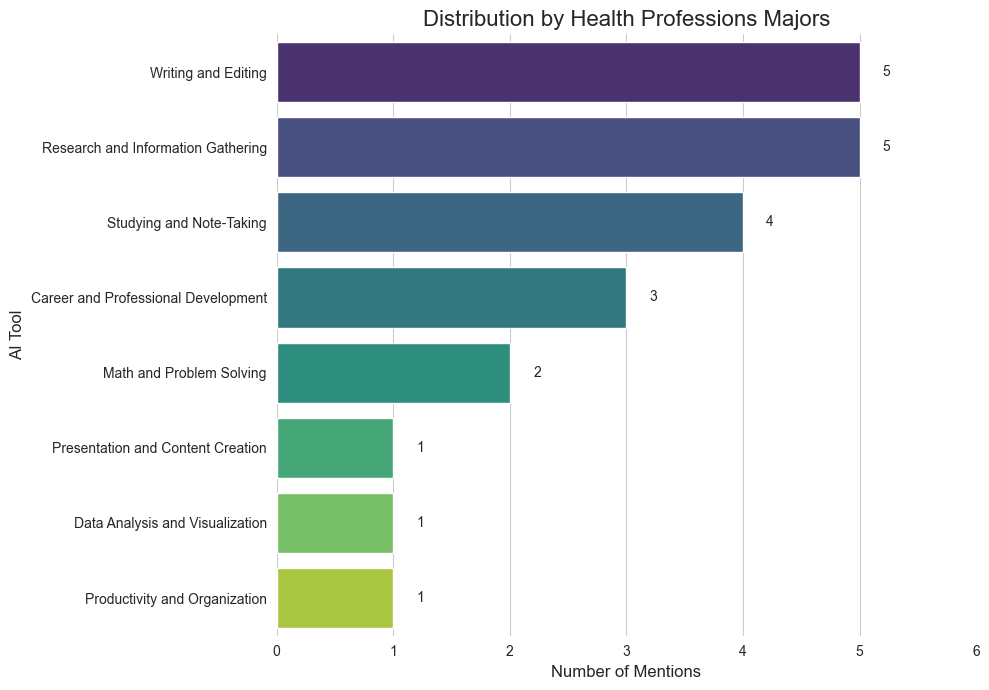
\includegraphics[width=\textwidth]{fig6-4.png} % Replace with your second subfigure file name
    %\caption{Description of subfigure (b)}
    \label{fig:subfig1b}
  \end{subfigure}
  \caption{Overall caption for the two subfigures.}
  \label{fig:subfigures1}
\end{figure}


The survey also included three attitudinal statements rated on a five-point Likert scale. In response to “AI improves my learning experience as a student,” 19 participants strongly agreed, 13 somewhat agreed, 4 neither agreed nor disagreed, 2 somewhat disagreed, and 1 strongly disagreed (Figure 11).

\begin{figure}[htbp]
  \centering
  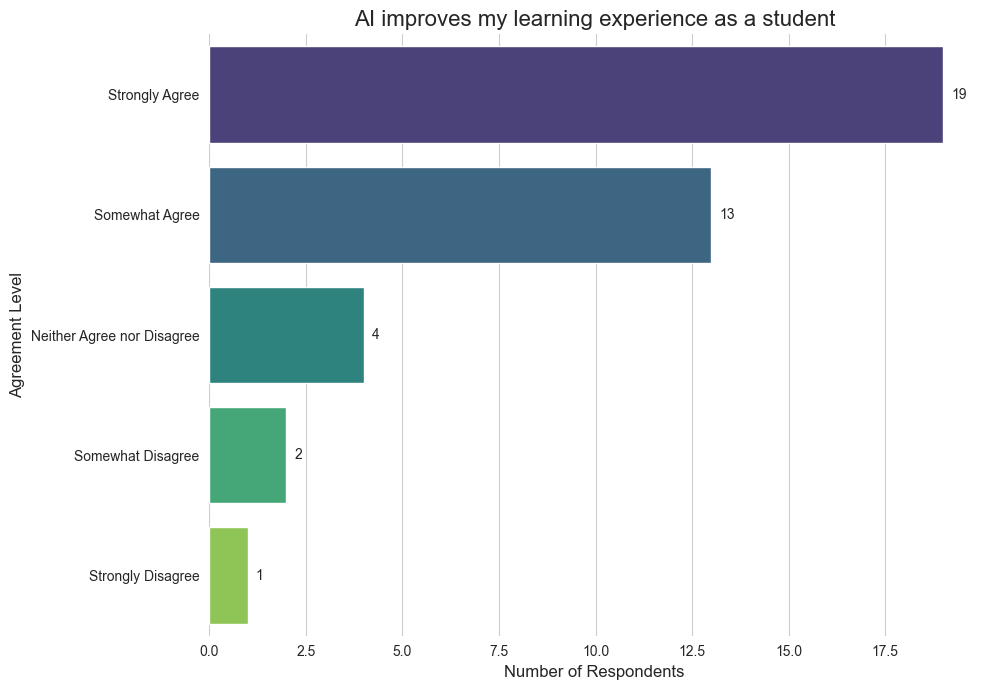
\includegraphics[width=0.65\textwidth]{fig7-1.png} % Replace with your figure file name
  \caption{A brief description of the figure.}
  \label{fig:example1}
\end{figure}

For “AI tools are accessible to me,” responses were predominantly positive: 23 strongly agreed, 15 somewhat agreed, and 2 neither agreed nor disagreed (Figure 12).

\begin{figure}[htbp]
  \centering
  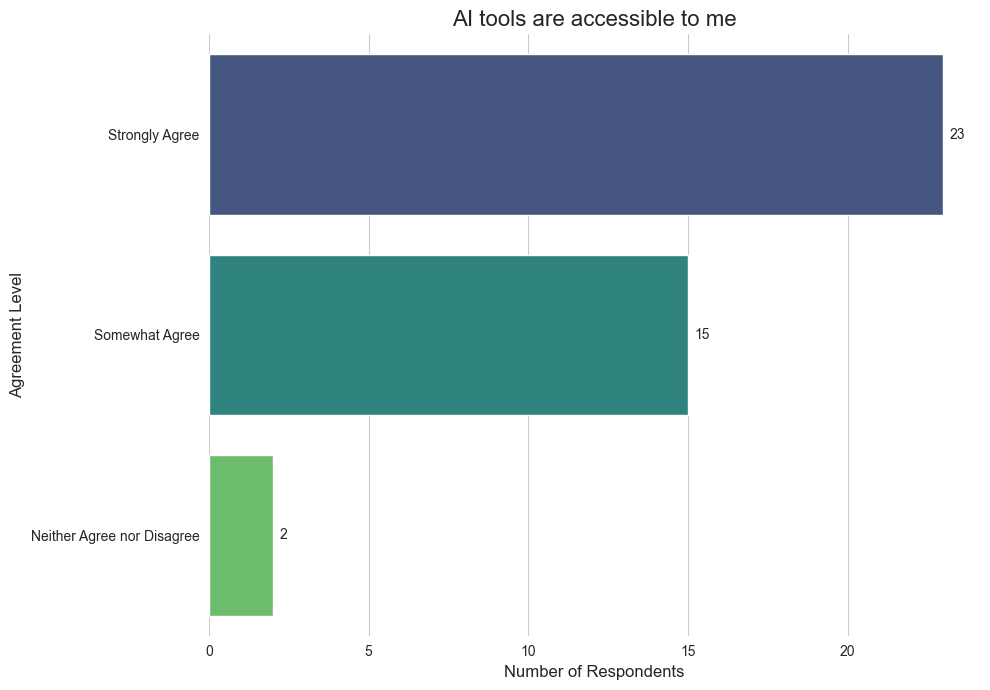
\includegraphics[width=0.8\textwidth]{fig7-2.png} % Replace with your figure file name
  \caption{A brief description of the figure.}
  \label{fig:example1}
\end{figure}

The final statement, “AI tools are more beneficial in my field of study compared to others,” yielded more mixed results: 17 selected “neither agree nor disagree,” 10 somewhat agreed, 9 strongly agreed, and 4 somewhat disagreed (Figure 13).

\begin{figure}[htbp]
  \centering
  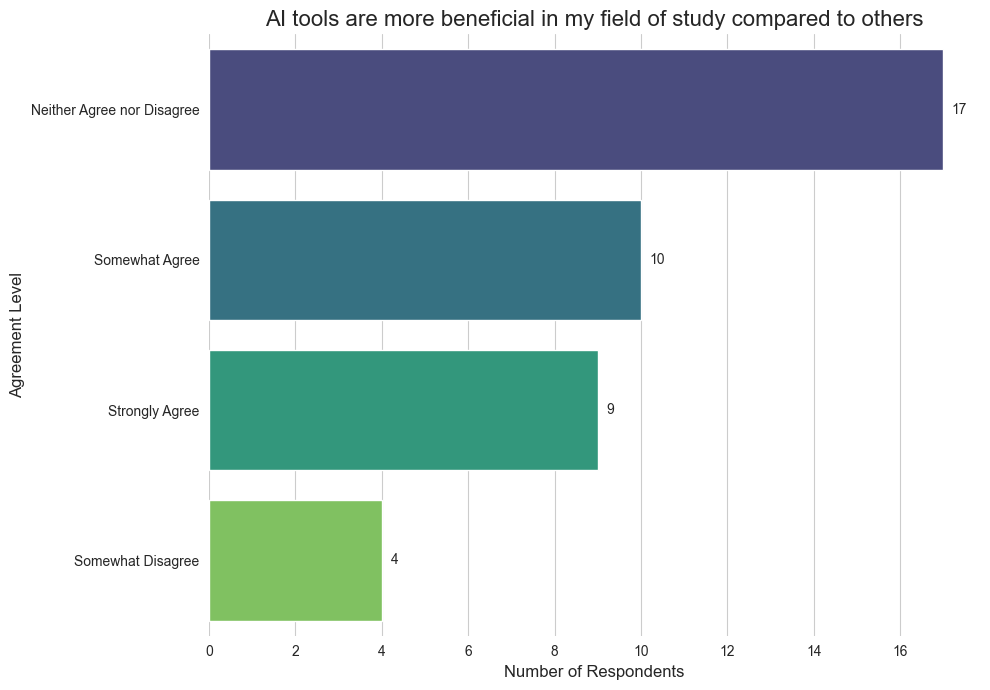
\includegraphics[width=0.8\textwidth]{fig7-3.png} % Replace with your figure file name
  \caption{A brief description of the figure.}
  \label{fig:example1}
\end{figure}

A more detailed analysis of attitudinal differences by academic field is presented in the Discussion and Conclusion section.

\subsection{Textual Description of Results}
Describe the main findings in words.

\subsection{Figures}
\label{subsec:figures}
You can include figures in this subsection or create separate subsections for different sets of figures.

% Example of a single figure
\begin{figure}[htbp]
  \centering
  \includegraphics[width=0.7\textwidth]{example-image-a} % Replace with your figure file name
  \caption{A brief description of the figure.}
  \label{fig:example1}
\end{figure}

% Example of two subfigures side-by-side
\begin{figure}[htbp]
  \centering
  \begin{subfigure}[b]{0.45\textwidth}
    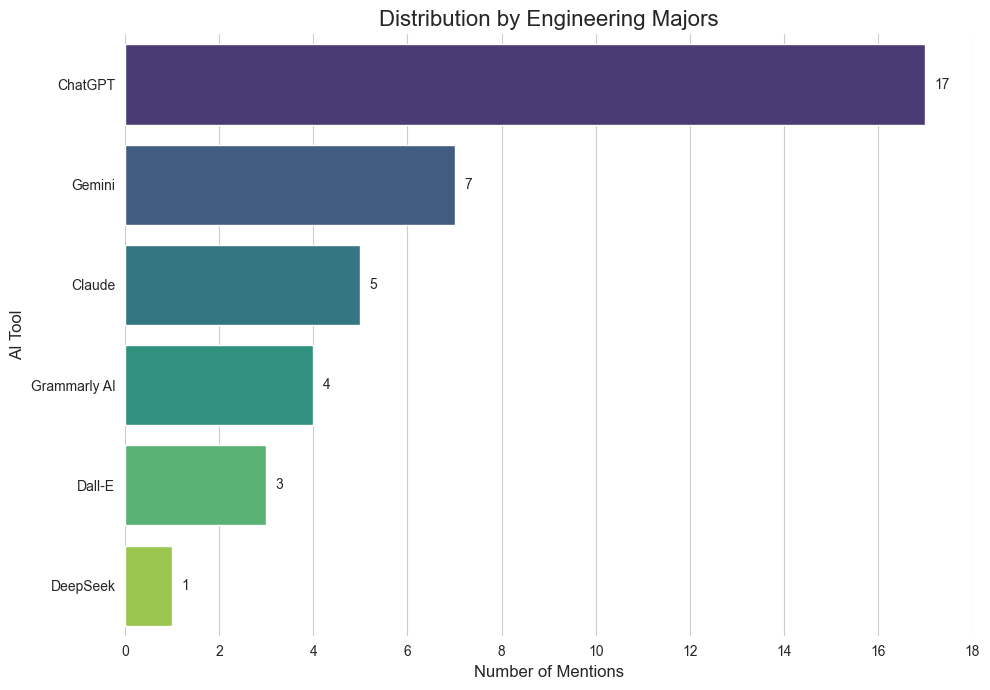
\includegraphics[width=\textwidth]{fig4-1.png} % Replace with your first subfigure file name
    \caption{Description of subfigure (a)}
    \label{fig:subfig1a}
  \end{subfigure}
  \hfill % Add some horizontal space between the subfigures
  \begin{subfigure}[b]{0.45\textwidth}
    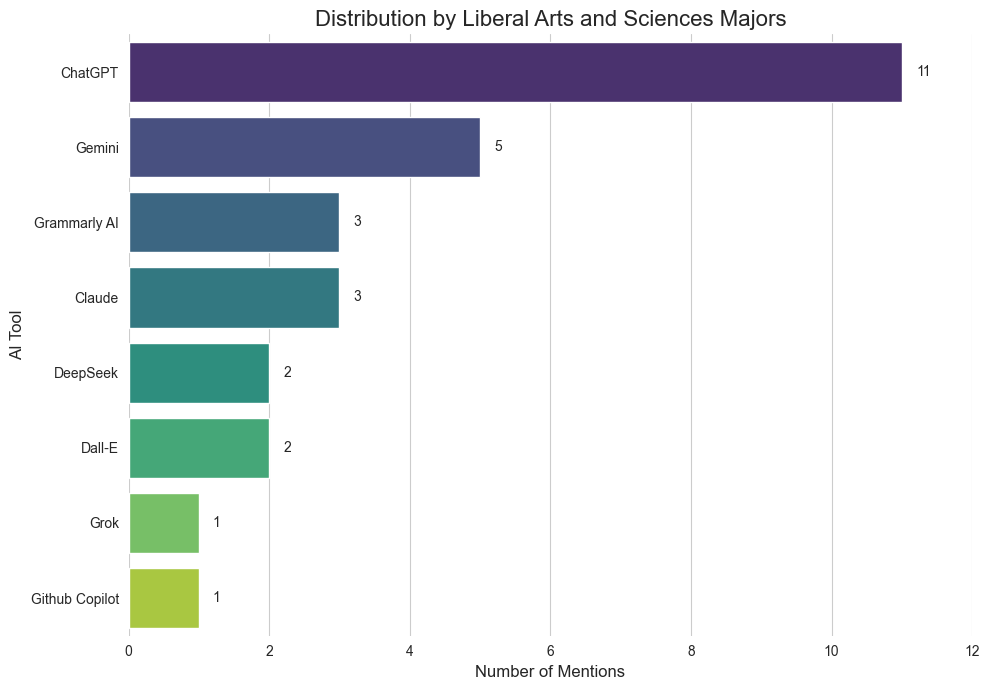
\includegraphics[width=\textwidth]{fig4-2.png} % Replace with your second subfigure file name
    \caption{Description of subfigure (b)}
    \label{fig:subfig1b}
  \end{subfigure}
  \hfill % Add some horizontal space between the subfigures
  \begin{subfigure}[b]{0.45\textwidth}
    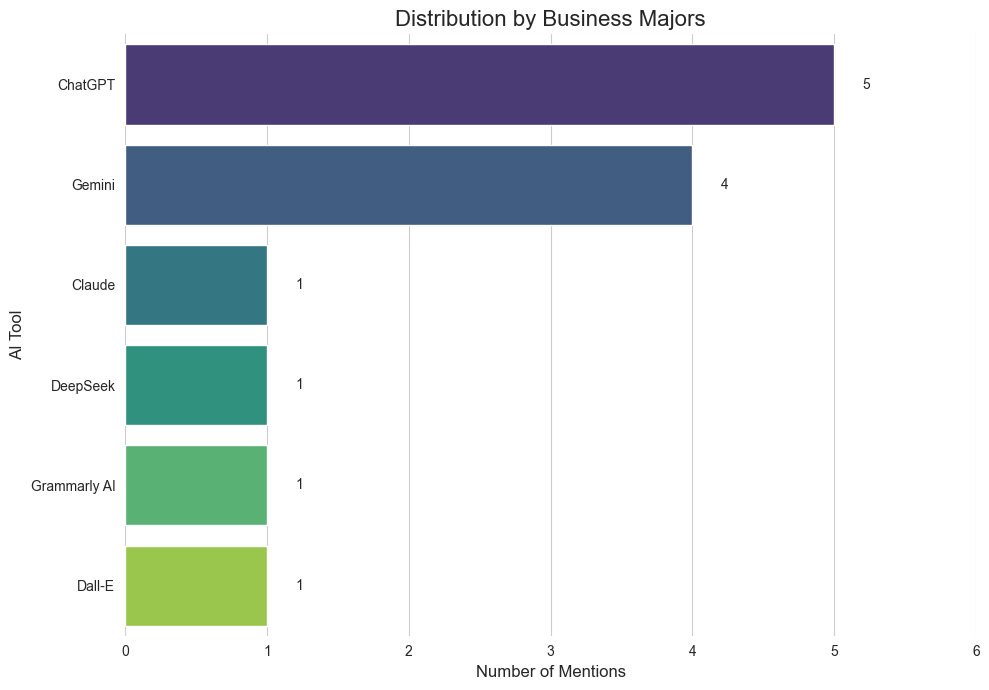
\includegraphics[width=\textwidth]{fig4-3.png} % Replace with your second subfigure file name
    \caption{Description of subfigure (b)}
    \label{fig:subfig1b}
  \end{subfigure}
  \hfill % Add some horizontal space between the subfigures
  \begin{subfigure}[b]{0.45\textwidth}
    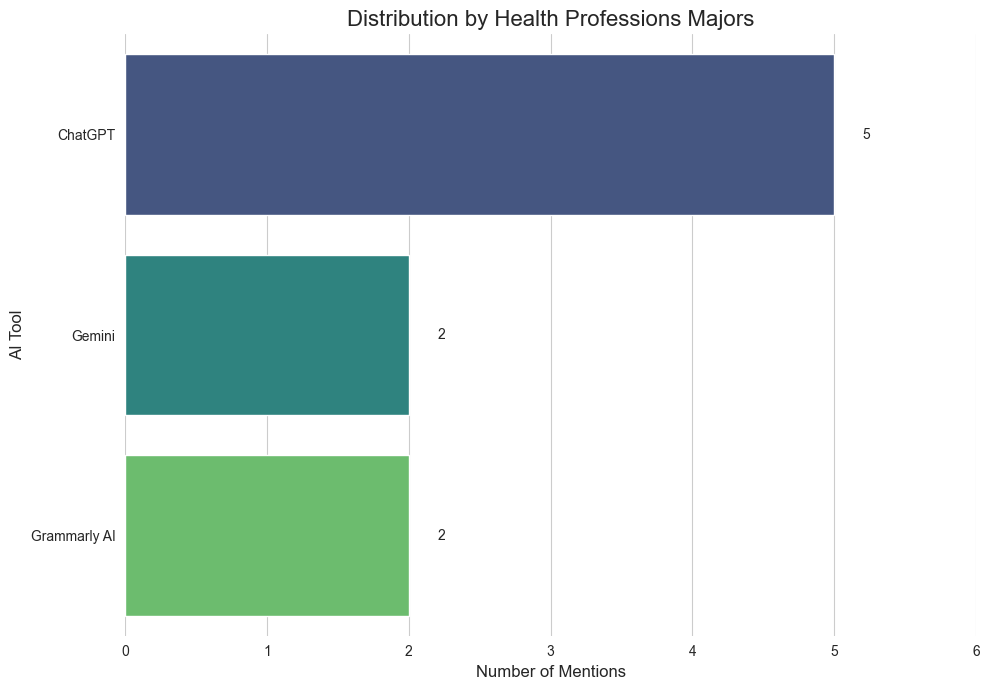
\includegraphics[width=\textwidth]{fig4-4.png} % Replace with your second subfigure file name
    \caption{Description of subfigure (b)}
    \label{fig:subfig1b}
  \end{subfigure}
  \caption{Overall caption for the two subfigures.}
  \label{fig:subfigures1}
\end{figure}

% --- Discussion ---
\section{Discussion}
\label{sec:discussion}
In this section, you interpret and discuss the results presented in the previous section. Relate your findings back to the research question and the existing literature. Discuss the implications of your findings, any limitations of your study, and potential avenues for future research.

% --- Conclusion ---
\section{Conclusion}
\label{sec:conclusion}
Summarize the main findings and conclusions of your research. Briefly reiterate the significance of your work.

% --- Acknowledgements (Optional) ---
\section*{Acknowledgements}
You can acknowledge individuals or organizations that provided support for your research.

% --- References ---
\section*{References}
\label{sec:references}
List all the sources you cited in your report using a consistent citation style.

% Example using a simple \thebibliography environment:
\begin{thebibliography}{99}
  \bibitem{AuthorYear} Author, A. (Year). \textit{Title of the book or article}. Publisher or Journal Name, Volume(Issue), pages.
  % Add more references here
\end{thebibliography}

% --- Appendices (Optional) ---
\appendix
\section{Appendix A: Supplementary Material}
Include any supplementary materials here.

% --- End Document ---
\end{document}